\section{HiFi-forstærkerens generelle opbygning}

En HiFi-forstærker kan være opbygget på forskellige måder, som blandt andet er afhængig af kravene til indgangstyper, THD og strømforbrug. Derudover kan forskellige designs variere alt efter hvilke funktioner der inkluderes, såsom; volumenkontrol, equalizer, mixer, fjernbetjening og lignende. 
En HiFi-forstærker kan. som sagt, designes på forskellige måder alt efter ydelse og funktioner. Et eksempel på en måde at opbygge en forstærker på er vist på figur \ref{fig:forstaerker_opbygning}.

\begin{figure}[h]
\centering
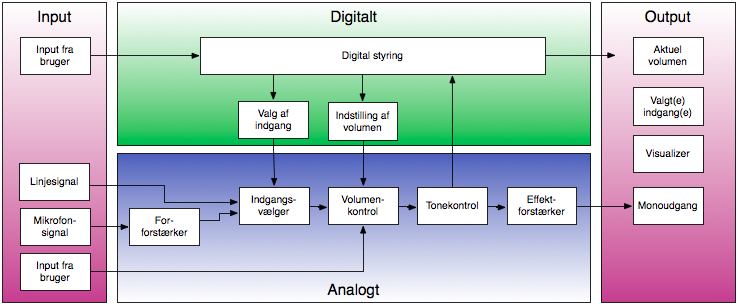
\includegraphics[scale=.6]{indledende_analyse/generel_effektforstaerker/forstaerker_opbygning.png}
\caption{Opbygning af HiFi-forstærker}
\label{fig:forstaerker_opbygning}
\end{figure}

Der er i ovenstående eksempel medtaget funktionerne: Volumenkontrol, equalizer, visualizer, display og fjernbetjening. En del af HiFi-forstærkeren kan designes med digital elektronik og en del med analog. \fixme{Hvad i alverden skal jeg skrive? Det bliver noget pladder?}